\chapter{Tutorial}

\section{Preconditions}




\section{Creating a productline}
Enter the command 'newpl'. A listing is shown with the properties of the lately created
productline. You can change the properties as described above. By enetering 'p' the SAT
tries to create a new productline with the current settings. \par

Please not that every productline of a Kobold server must have an unique name. Creation
of a productline with an already assigned name will be refused by the server.



\section{Creating a new user}
Enter the command 'newuser'. A listing is shown with the properties of the lately created
user, his/her username, fullname and initial password. After enetering 'p' a new user with
the shown properties is created on the server.\par

Note that every registered user needs to have its own unique username. Creation of a new user 
with a username that's already been registered will be refused by the server.



\section{Assigning an existing user to a productline as PLE}
Enter the command 'assignple'. You are asked to enter the name of the person you want
to become PLE. Finally, enter the name of the productline you want to assign the new 
PLE to. Once you confirmed your entry, the user has PLE rights.


\section{Starting a new project}

In the File menu select 'New' and then 'Kobold PLAM Project'. The Kobold wizard opens.
Enter the url of your Kobold server, your username and password. Then press
"test connection". If the test succeeds, the "next" button is enabled (see \ref{wizard1}).

\begin{figure}[h!]
\begin{center}
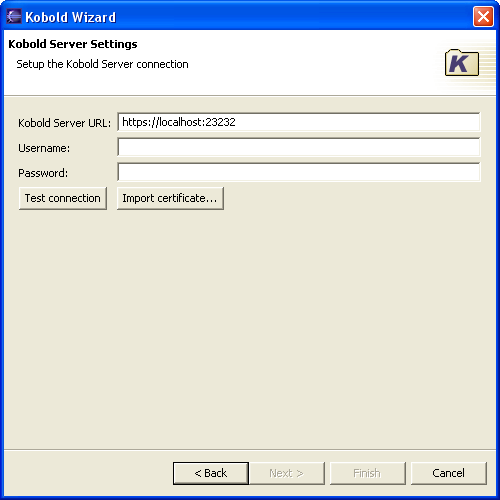
\includegraphics[width=10cm]{wizard1.png}
   \caption{Kobold wizard}
\label{wizard1}
\end{center}
\end{figure}\par

After that you choose the productline you want to check out (see \ref{wizard2}).

\begin{figure}[h!]
\begin{center}

\includegraphics[width=10cm]{wizard2.png}
   \caption{Kobold wizard}
\label{wizard2}
\end{center}
\end{figure}\par

In the last step you have to enter the name of the project you want to create (see \ref{wizard3}).

\begin{figure}[h!]
\begin{center}
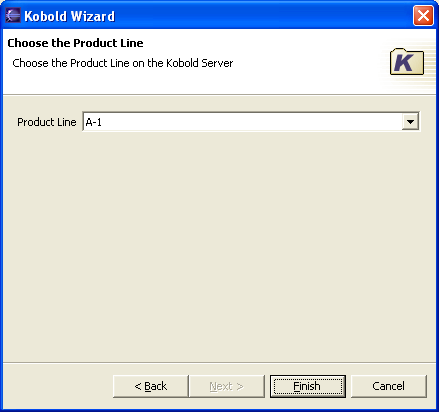
\includegraphics[width=10cm]{wizard3.png}
   \caption{Kobold wizard}
\label{wizard3}
\end{center}
\end{figure}\par

A new project has been created. You can open the different views through the Window menu
and 'show view'. 

\section{Creating a Core Assets}

In the pallete select the "component" item. Click within a variant or top-level in 
the Architecture Editor. A component is inserted (see \ref{component}) and a dialog opens where you can enter the meta data of
the component. Per drag+drop you can simply change the size of the component. \par
Note: Core Assets/Components can only be inserted top-level or into variants.

\begin{figure}[h!]
\begin{center}

\includegraphics[width=8cm]{component.png}
   \caption{Component}
\label{component}
\end{center}
\end{figure}\par


\section{Creating variants}

In the pallete select the "variant" item. Click within a component in 
the Architecture Editor. A variant is inserted (see \ref{variant}) and a dialog opens where you can enter the meta data of
the variant. Per drag+drop you can simply change the size of the variant. \par
Note: Variants can only be inserted into components.

\begin{figure}[h!]
\begin{center}

\includegraphics[width=10cm]{variant.png}
   \caption{Variant}
\label{variant}
\end{center}
\end{figure}\par


\section{Creating releases}

In the pallete select the "release" item. Click within a variant in 
the Architecture Editor. A release is inserted (see \ref{release}) and a dialog opens where you can enter the meta data of
the release. For each file of the variant you can select the revision number you want to add to the release. 
Per drag+drop you can simply change the size of the release. \par
Note: Releases can only be inserted into variants.

\begin{figure}[h!]
\begin{center}

\includegraphics[width=10cm]{release.png}
   \caption{Release}
\label{release}
\end{center}
\end{figure}\par




\section{Creating a dependency edge}

In the pallete select the "include edge" item. Select an item in the Architecture Editor
as the starting point. The next item you select will be the aiming point (see \ref{include}).

\begin{figure}[h!]
\begin{center}

\includegraphics[width=10cm]{include.png}
   \caption{Dependency edge}
\label{include}
\end{center}
\end{figure}\par



\section{Creating a product}

In the palette press 'compose product'. The components, etc. in the architecture view turn
grey. You can now select the components, variants and releases you want to include into
you new product. The chosen objects turn blue (see \ref{compose}). When done press the 
'create product' button in the Architecture Editor. A dialog opens where you can enter
the name and metainfo of your new product. After confirming the dialog, you can see
your new product in the Architecture Tree and Architecture Editor

\begin{figure}[h!]
\begin{center}

\includegraphics[width=10cm]{composeproduct.png}
   \caption{Composing a Product}
\label{compose}
\end{center}
\end{figure}\par





\section{Writing a mail}

In the menu of the Workflow View select "new mail". A Workflow window opens where
you can enter your message, the subject and the recipient of the message. Send the
message by pressing the "Send" button. Pressing the "Cancel" button will close the window
without sending your message (see \ref{writemail}).

\begin{figure}[h!]
\begin{center}
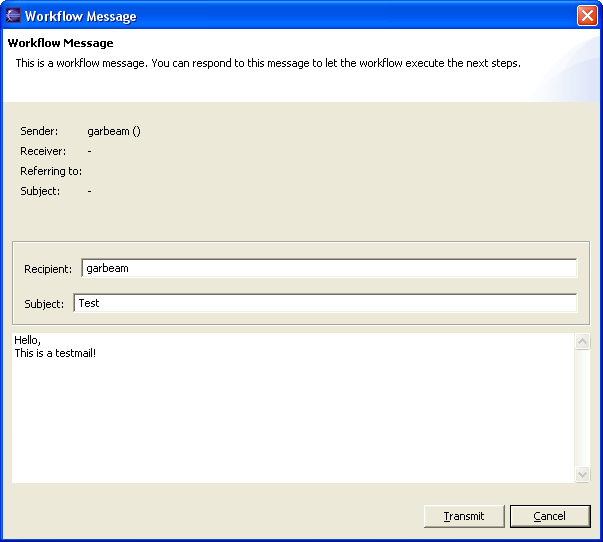
\includegraphics[width=10cm]{writemail.png}
   \caption{Write a new mail}
\label{writemail}
\end{center}
\end{figure}\par

\section{Answering a mail}

In the Workflow View double-click on the mail you want to answer. A Workflow
window opens where you can see the message text of the mail. Below you can enter
the subject and the text of your reply. Send the answer by pressing the "Send" 
button. Pressing the "Cancel" button will close the window without sending 
your message (see \ref{answermail}).

\begin{figure}[h!]
\begin{center}
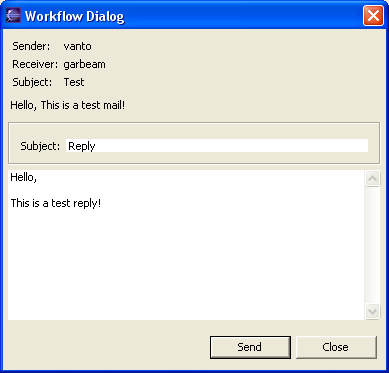
\includegraphics[width=10cm]{answermail.png}
   \caption{Answer a mail}
\label{answermail}
\end{center}
\end{figure}\par







